% ----------------------------------------------------------------------------------
% Kapitel: Fundamentals and Key Terminologies 5
% ----------------------------------------------------------------------------------
\subsection{Fundamentals of Anomaly Detection}
In the previous chapter, a closer look was taken at what Artificial Intelligence is and how useful it can be in the field of EVSEs. In this chapter, the focus is on the area of Anomaly Detection and its fundamental concepts.\\
Anomaly Detection is the process of analyzing data patterns to identify outliers. Data points deviate significantly from the norm. This technique can be applied in a wide range of domains, including credit card fraud detection, insurance and healthcare monitoring, intrusion detection in cybersecurity, fault detection in safety-critical systems, military surveillance, and also in the field of EVSEs \cite{paper_AnomalyDetection_Northwestern}.\\
Outliers are data points that differ significantly from the majority of the data. In the paper by Hodge and Austin, they define outliers as "data points that are inconsistent with the rest of the data". The paper also includes some informative figures that illustrate the different types of outliers and how they can be detected \cite{paper_HodgeAustin}.\\
\begin{figure}[H]
  \centering
  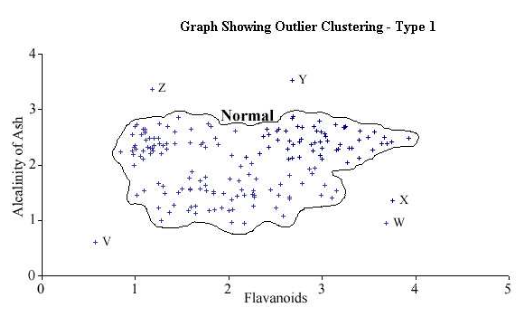
\includegraphics[width=0.5\textwidth]{pics/outlier_clustering_type1.png}
  \caption{Data distribution classified by Type 1: Outlier Clustering \cite{paper_HodgeAustin}.}
  \label{fig:outlier_clustering_type1}
\end{figure}
Type 1 is the most common form of outlier, data points are generally clustered around a central value, but a few points differ significantly from the rest. This can be seen in the Figure~\ref{fig:outlier_clustering_type1}, where most data is centered, yet a few outliers deviate clearly.\\
Such outliers can be detected using a simple Z-score algorithm, where the mean $\mu$ and the standard deviation $\sigma$ of the data are calculated. The Z-score is computed using the formula: $Z = \frac{X - \mu}{\sigma}$. Estimated Z-scores greater than 3 or less than -3 can be considered anomalies. These anomalies should be given increased attention during data analysis. Additionally, anomalies can be contextualized by parameters such as time or location to improve their identification \cite{paper_IJITEE_z_score}.
\begin{figure}[H]
  \centering
  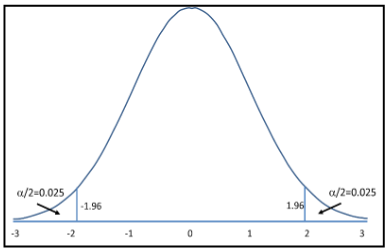
\includegraphics[width=0.4\textwidth]{pics/z_score.png}
  \caption{Z-score with critical region \cite{paper_IJITEE_z_score}}
  \label{fig:z_score}
\end{figure}
Before the Z-score can be calculated, extensive data collection and preprocessing are required. This forms the first step in the Anomaly Detection process. The data must be cleaned, normalized, and transformed to ensure that its suitable for analysis. This may involve removing duplicates, handling missing values, and scaling the data to a common range.\\
After the data is preprocessed, feature engineering is performed to extract relevant features from the data. Feature engineering involves selecting and transforming the data and can sometimes also include the creation of new features that improve the performance of the anomaly detection model. Data reduction is also a relevant step in this process, where the data is reduced to a smaller set of features that are most relevant for the anomaly detection task \cite{maharana2022review}.\\
Once data collection and preprocessing are completed, a suitable model must be selected for the specific anomaly detection case. Before analyzing the different models, it is important to examine the typical challenges associated with anomaly detection.\\
As previously mentioned, detecting anomalies requires analyzing data patterns to identify outliers. Determining the correct boundary between normal and abnormal data is challenging and highly dependent on the context.\\
The EVSE infrastructure changes rapidly. This happens not only due to new technologies, charging stations also change with every new charging process and through communication with other stations in the network. This variability makes it difficult to define a static outlier threshold. Therefore, it is essential to adapt the anomaly detection model to the current state of the EVSE network and the ongoing charging processes. This enables dynamic detection capabilities that remain effective under all conditions in a highly dynamic EVSE environment \cite{paper_AnomalyDetection_Northwestern}.\\
